\section{Introduction}
The current dominant approach for language modeling is based on \gls{ntpar} training. \Gls{ntp} language models learn the conditional distribution of the \textit{next token} given the previous tokens in a sequence \citep{shannon1951prediction,radford2019language}. The resulting language model is sampled auto-regressively left-to-right, one token at a time.
Recent work proposes \glspl{mdlm} \citep{austin2021structured,sahoo2024simple,shi2024simplified} as an alternative to \gls{ntpar} models.  
\glspl{mdlm} are trained to in-fill sequences with randomly masked positions. The resulting model learns the distribution $p_\theta(x^i | \mbx_{\textsc{un-masked}})$ at every masked position $i$. 



\begin{figure*}[ht]
    \centering
    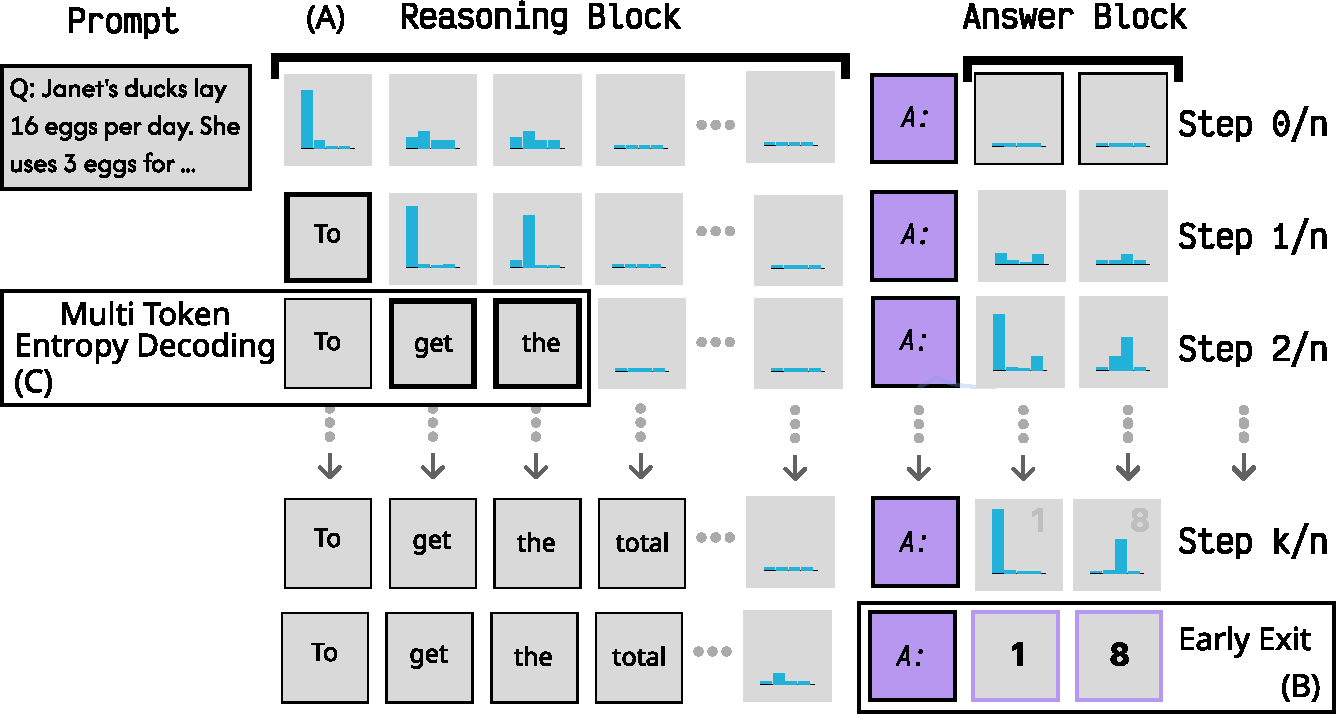
\includegraphics[width=0.80\linewidth]{method_fig.pdf}
    \caption{\glspl{mdlm} learn the conditional distributions at each masked token position. A) We reframe reasoning as infilling a prompted reasoning template, which enables directly modeling answer token probabilities \textit{during} reasoning. This provides several benefits, like B) enabling early exits or \textit{post-hoc} reasoning given a pre-filled answer. C) We also utilize the entropy of these distributions to adaptively set the number of tokens decoded at each step. 
    }
    \label{fig:reasoning_template}
\end{figure*}

While modeling all masked positions requires additional effort, \glspl{mdlm} have several potential benefits, such as parallel token decoding \citep{sahoo2024simple,sahoo2025esoteric}, and flexible decoding orders \citep{kim2025train} that lead to significant improvements on logic puzzles, such as Sudoku. Additionally, \citet{bachmann2024pitfalls,prabhudesai2025diffusion}
show that multi-token prediction objectives can achieve better likelihoods and accuracy on tasks,
and access to the distribution and samples from masked positions supports controllable generation \citep{schiff2024simple,singhal2025generalframeworkinferencetimescaling}.

In our work, we first examine two purported benefits of \glspl{mdlm}: any-order and multi-token decoding, on mathematical reasoning and coding benchmarks. Despite the flexibility enabled by \glspl{mdlm}, 
we observe that decoding one token in a left-to-right order, identically to an \gls{ntp} model, is a strong decoding choice for
\gls{mdlm} models. Even decoding just two tokens in parallel substantially reduces performance on popular benchmarks. These findings raise questions about the substantial extra compute \glspl{mdlm} spend to model the distribution of all masked positions.
In this work,  we show how this compute can be made \textit{useful}. We demonstrate that the access that \glspl{mdlm} provide to the conditional distributions of all masked positions, and their ability to in-fill, unlocks new sampling and post-training capabilities that are not readily available for \gls{ntp} models. 


First, we demonstrate that the ability of \gls{mdlm} to in-fill opens up new model prompting paradigms. In this work, we propose prompting-as-infilling, where we add user-specified contexts in multiple positions, not just the beginning of the sequence, unlike \gls{ntp} models. Specifically, we consider \textbf{{reasoning-as-infilling}}. Here we pre-fill an explicit reasoning template, with specific reasoning and answer positions (see \cref{fig:reasoning_template}).
This enables sampling reasoning traces conditioned on a reasoning budget and format. 
We demonstrate that the in-filled template provides many advantages. 
By explicitly distinguishing token answer positions, we can make use of the conditional distributions of the masked positions provided by \glspl{mdlm} to measure the uncertainty of the answer \textit{while reasoning}. In turn, this enables \textbf{early exits} once the model converges on an answer, reducing inference costs. For instance, on \textsc{gsm8}k this leads to $24\%$ fewer function calls with no degradation in accuracy. 

{{Reasoning-as-infilling}} has consequences for analyzing model behavior and improving performance. Given access to an answer, we can sample from the \gls{mdlm}'s posterior distribution of reasoning traces conditioned on the answer, $p_\theta(\mbr \mid \mbc, \mba)$. This easy sampling from the posterior in \glspl{mdlm} enables generating high-quality \textit{post-hoc} reasoning traces for use in model fine-tuning.

Next, we revisit multi-token decoding. Decoding multiple positions in a single step results in samples that are not from the \gls{mdlm}'s learned distribution, as typically the joint distribution and factorized distributions do not align, $p_\theta(x^i, x^j \mid \mbx_{\textsc{un-masked}}) \neq p_\theta(x^i \mid \mbx_{\textsc{un-masked}}) p_\theta(x^j \mid \mbx_{\textsc{un-masked}})$. However, by making use of the entropy of the masked positions to inform decoding, we can control how much multi-token decoding deviates from single token sampling. We propose Multi-token Entropy Decoding (\textsc{med}), an \textbf{adaptive multi-token decoder} that decodes multiple positions only if the conditional entropy of the additional positions falls below a specified threshold. We find that \gls{med} leads to $2$-$3\times$ fewer function calls, with a minor or no drop in performance. 



\paragraph{Contributions.} In this paper, we:
\begin{itemize}[leftmargin=*]
    \item Evaluate \gls{mdlm} models, such as Dream \citep{Dreamon2025} and LLaDA \citep{nie2025largelanguagediffusionmodels}, on several tasks and find that the any-order sampling capability of \gls{mdlm} provides limited benefits on coding and mathematical reasoning benchmarks, and that standard multi-token decoding degrades performance.
    \item Introduce {reasoning-as-infilling} for \glspl{mdlm}, which leverages their infilling capabilities. We then show that distinguishing reasoning and answer tokens can provide several benefits, such as:
    \begin{itemize}[leftmargin=*]
        \item \textit{Early exits}, where if the model is certain about the answer, we then skip the remaining reasoning steps. This leads to a $3.3\times$ speed when combined with multi-token entropy decoding (\gls{med}). 
        \item \textit{Post-hoc reasoning}, where given question-answer pairs, we generate reasoning traces conditioned on the answer. On the \textsc{gsm8}k dataset, we find that supervised fine-tuning on these reasoning traces can improve the model more than supervised fine-tuning on the \textit{human-annotated} \textsc{gsm8}k reasoning traces.         
                
        \item \textit{Scoring reasoning traces}, where given an answer, we can score the reasoning process for correctness at intermediate steps using the distributions of the answer block, without an external verifier or roll-outs. These scores correlate with whether the reasoning steps lead to a correct answer. 
    \end{itemize}
        
    \item Propose \gls{med}, an adaptive sampler that provides a $2$-$3\times$ speed-up, without any loss in performance on math and coding benchmarks.    
\end{itemize}








   

\section{Related Work}
\paragraph{Multi-Token Prediction and Speculative Decoding.}
\citet{gloeckle2024better} show that models trained with the multi-token objective can enable parallel multi-token decoding, or \textit{speculative decoding}, without making use of another model. However, unlike \glspl{mdlm}, \citet{gloeckle2024better} limit to predicting the next $2, 4$ tokens. Several other works \citep{leviathan2023fast,chen2023accelerating} show that using smaller draft models for generation and then rejection sampling can also enable parallel decoding with \gls{ntp} models. However, \glspl{mdlm} offer many possibilities beyond left-to-right parallel decoding, such as in-filling, and error correction through re-masking of unmasked tokens \citep{wang2025remasking}. \citet{israel2025accelerating} propose an adaptive multi-token decoder which samples from the product of an \gls{ntp} and \gls{mdlm} model. Unlike \gls{med}, their approach relies on rejection sampling based on an external \gls{ntp} model. 


\citet{ben2025accelerated} propose entropy-bound (\textsc{eb}) sampler, an adaptive multi-token decoder for \glspl{mdlm}, which similar to \gls{med} controls the error incurred by multi-token decoding. \textsc{eb} sampler adds multiple positions to unmask based on the difference between the sum of the positions added and the maximum entropy until the difference exceeds a specified threshold $\gamma$. \gls{med} unmasks positions based on the individual entropies rather than thresholding based on the sum. We observe that \gls{med} leads to fewer \textsc{nfe}s while getting higher accuracies, see tables 6 and 7 in \citet{ben2025accelerated} versus \cref{tab:early_exit_combined} for a comparison. \citet{wu2025fast} propose accelerating inference with \glspl{mdlm} using \textsc{kv}-caching and parallel decoding. 
Similar to \citet{ben2025accelerated}, they propose an adaptive greedy strategy, instead decoding tokens with confidences above a fixed probability threshold, unlike \gls{med}, which thresholds based on entropy. Additionally, the method proposed in \citet{wu2025fast} is designed to accelerate $\arg \max$ sampling from \glspl{mdlm}, whereas \gls{med} is compatible with inference-time steering methods and post-training methods that require multiple samples per prompt, such as  \textsc{rloo} \citep{ahmadian2024back} and  \textsc{grpo} \citep{shao2024deepseekmath,zhao2025d1scalingreasoningdiffusion}.

\paragraph{Post-hoc Reasoning.}
\citet{zelikman2022star} proposes fine-tuning language models on reasoning traces that are generated conditioned on a correct answer. \citet{phan2023training,ruan2025reasoning} propose fine-tuning a model on samples from approximations of the posterior $p_\theta(\mbr \mid \mbc, \mba)$. In contrast, \glspl{mdlm} enable exact sampling from the posterior of the reasoning traces given the answer by simply in-filling the answer in the answer block provided in the {reasoning-as-infilling} framework.

\section{Masked Diffusion Language Models}
\Glspl{mdlm} \citep{sohl2015deep,devlin2019bert,austin2021structured,sahoo2024simple,shi2024simplified} are a class of generative models for modeling discrete data $\mbx \sim \qdata$, where $\mbx = (x^1, x^2, \dots, x^{L})$ and each position $x^i$ takes values in a finite vocabulary $\mathcal{V}$. For training the model $p_\theta(\mbx \mid \mbc)$, the sequence $\mbx \sim \qdata$ is masked randomly and the model learns to predict the distributions of the masked positions for a fixed length sequence by maximizing:
\begin{align}\label{eq:likelihood_bound}
 \cL(\mbx, \mbc, \theta): = \E_{\textsc{masked-set} \sim U}  \sum_{j \in \textsc{masked-set}}  \log p_\theta( x^j \mid \mbx_{\textsc{un-masked}}, \mbc)
\end{align}
where $\textsc{masked-set}$ is a set of randomly masked positions in $\{1, 2, \dots, L\} $. Sampling from an \gls{mdlm} is performed by iteratively un-masking positions. Notably, an \gls{mdlm} can also  be viewed as any-order auto-regressive model \citep{uria2014deep,ou2024your}, where given a decoding order $\mbo = [o_1, \dots, o_L]$ with $o_j \in \{1, 2, \dots, L \}$, the sampling model can be defined as:
\begin{align}
    p_\theta(\mbx \mid \mbc, \mbo) = \prod_{j=0}^{L-1} p_\theta(x^{o(j)} \mid \mbx_{o(<j)}, \mbc) 
\end{align}
where $o_j$ refers to the position decoded at step $j$ and $\mbx_{o(<j)}$ refers to all positions decoded prior to step $j$. Additionally, block-sampling \citep{sahoo2024simple,nie2025largelanguagediffusionmodels,arriola2025blockdiffusioninterpolatingautoregressive} approaches define a left-to-right sequence of fixed length blocks and decode within each block in  an arbitrary order. 
\begin{figure*}[t]
    \centering
    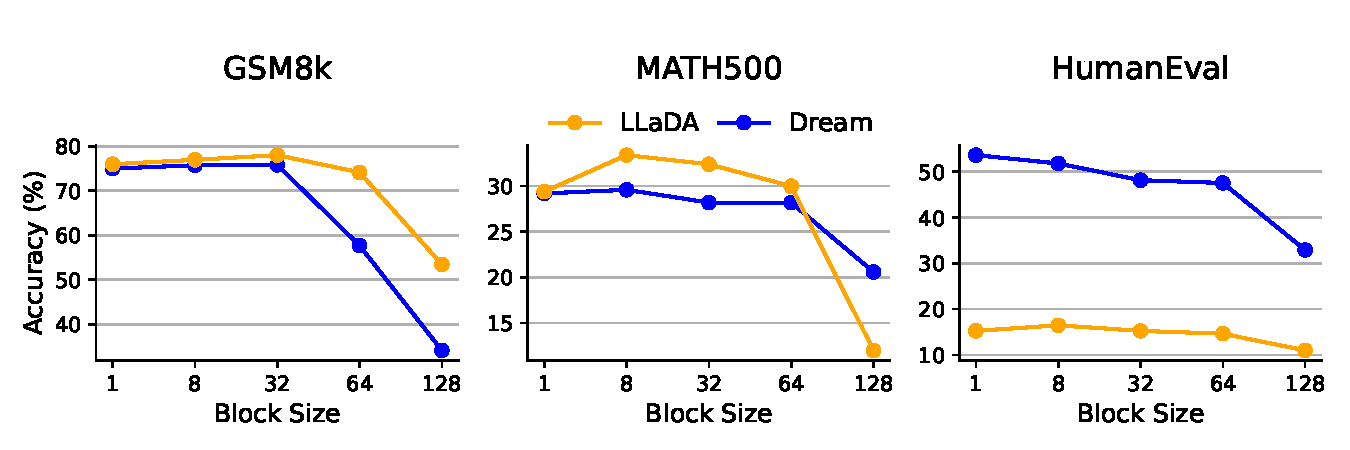
\includegraphics[width=\linewidth]{plots/performance_comparison.pdf}
    \caption{\textbf{Left-to-right sampling with \glspl{mdlm} is a competitive sampling algorithm for reasoning and coding.} When performing entropy decoding \citep{ye2025dream}, we observe that full any-order sampling results in poor performance on all tasks but Sudoku. Left-to-right block decoding is required to make any-order sampling performant, and left-to-right sampling (block size $=1$) is always within a few percent of the best configuration. We also observe in \cref{tab:decoding_strategies} in \cref{appsec:observations} that performant block any-order configurations sample a large portion of tokens left-to-right. We consider sequences of length $128$.} 
    \label{fig:decoding_strategies}
\end{figure*}

\subsection{Preliminary Observations}
In our work, we first examine two purported benefits of \glspl{mdlm}: \textit{any-order} and \textit{multi-token} decoding, on popular mathematical reasoning, \textsc{gsm8}k \citep{cobbe2021trainingverifierssolvemath} and \textsc{math500} \citep{luo2024improve}, and coding benchmarks, \textsc{HumanEval} \citep{chen2021evaluating} as well as Sudoku \citep{sudokuLLM}:
\begin{enumerate}[leftmargin=*]
    \item \textbf{Does any-order decoding help for text?} Popular sampling  approaches for \glspl{mdlm} select positions to unmask based on confidence (e.g. token probability \citep{chang2022maskgit} or entropy \citep{kim2025train,ye2025dream}). We find that these any-order decoding algorithms either sample a large portion of tokens in a left-to-right order or underperform left-to-right sampling.  For example, on \textsc{gsm8}k, the best configuration of any-order entropy decoding samples $\sim 50\%$ of tokens left-to-right.
    Without block sizes \citep{arriola2025blockdiffusioninterpolatingautoregressive} that enforce a semi-\gls{ar} left-to-right structure, any-order significantly affects performance, see \cref{fig:decoding_strategies}.
    A notable exception where any-order sampling provides a significant benefit is Sudoku.
    We include additional analysis in \cref{appsec:observations} and in \cref{tab:decoding_strategies} in \cref{appsec:observations}. 

    \item \textbf{Does parallel decoding work?} We observe that even decoding two tokens in parallel at a time can severely hurt model performance across all tasks, see \cref{tab:parallel_decoding}. The resulting distributions also have high KL with respect to a one-token sampling algorithm, see \cref{tab:multi_token_kl}. 
\end{enumerate}

These findings show that the decoding order from \gls{ntp} models is performant for \gls{mdlm} models, despite their any-order and multi-token decoding capabilities. Despite these findings, we show that the additional capacities offered by \glspl{mdlm} have many possible benefits. 

\begin{table}[t]
    \centering
    \begin{tabular}{lcccccccc}
    \toprule
       \textbf{Parallel Tokens}  
       & \multicolumn{2}{c}{\textbf{GSM8K}} 
       & \multicolumn{2}{c}{\textbf{MATH500}}  
       & \multicolumn{2}{c}{\textbf{HumanEval}}  
       & \multicolumn{2}{c}{\textbf{Sudoku}} \\    
    \cmidrule(lr){2-3} \cmidrule(lr){4-5} \cmidrule(lr){6-7} \cmidrule(lr){8-9}
       & LLaDA & Dream 
       & LLaDA & Dream 
       & LLaDA & Dream 
       & LLaDA & Dream \\
    \midrule       
        1       & \textbf{76.95}  &  \textbf{75.73}  & \textbf{33.4}  & \textbf{29.6}  & \textbf{16.46}  & \textbf{51.82}  & 47.64 & \textbf{61.26} \\
        2       & 62.31  & 57.69  & 19.6  & 16.6  & 4.87  & 20.12  & \textbf{50.79} & 57.59 \\
        4       & 33.58  & 28.50  & 7.0   & 3.6   & 4.87  & 12.19  & 29.32  & 42.93 \\
    \bottomrule        
    \end{tabular}
    \caption{\textbf{\glspl{mdlm} can generate multiple fixed tokens in parallel, but this degrades accuracy.} We decode $1,2,4$ tokens in parallel, with block any-order (8) entropy decoding. We note that decoding even two tokens in parallel leads to a significant drop on all tasks but Sudoku.}
    \label{tab:parallel_decoding}
\end{table}
